\externaldocument{technical_work/ompss-2-integration.tex}

\section{Pthreads y mecanismos de sincronización}
\label{appendix:pthread}

En este apéndice se introduce superficialmente qué es un \textit{Pthread} y se hace hincapié en el mecanismo utilizado para la sincronización con las tareas registradas en \textit{Nanos6} con el modo librería introducido en la sección \ref{spawnfunction}
\bigskip

Históricamente los \textit{threads} se han implementado por cada fabricante o empresa, de una manera específica, complicando la portabilidad entre plataformas. Los \textit{Pthreads} nos proveen un estándar con la intención de que sea utilizado por la mayoría de máquinas. En todos los sistemas operativos del tipo \textit{UNIX} se implementan los \textit{threads} con el estándar \textit{IEEE POSIX 1003.1c}, y se les llama \textit{POSIX threads} o \textit{Pthreads}. El manual se puede encontrar en internet, y explica de lo más básico a lo más avanzado \cite{barney2009posix}. \todo{la cita ?}
\bigskip

Requerimos de un mecanismo de sincronización por que la función que se registra como tarea la ejecuta un \textit{thread} diferente al que la registra. 

\begin{figure}[H]
    \centering 
    \caption{Mecanismo de sincronización abstracto.}
    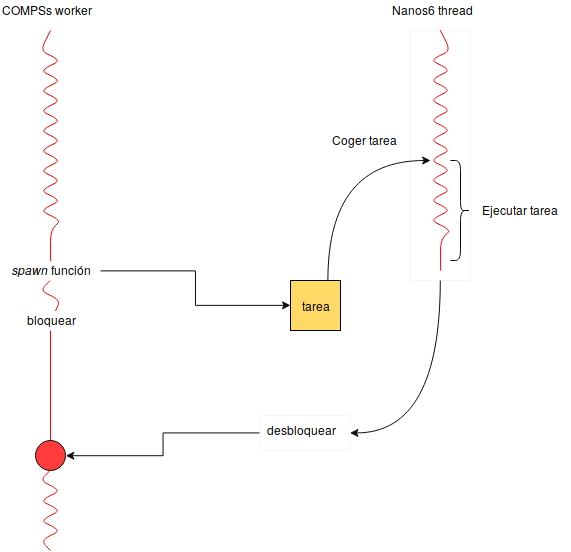
\includegraphics[scale=0.6]{spawn_sync.png}
    \label{fig:spawn_sync}
\end{figure}

En la figura anterior se muestran dos \textit{threads}, uno que registra una tarea y otro que espera a poder ejecutar alguna tarea. El primer \textit{thread} una vez haya registrado la tarea procederá a bloquearse, el segundo cuando acabe de ejecutar la tarea registrada, ejecutará un \textit{callback} donde desbloquearemos al primer \textit{thread}. \bigskip

El mecanismo abstracto es sencillo, pero la implementación real depende de los \textit{Pthreads}. Las estructuras utilizadas para realizar la sincronización son \texit{mutexes} y \textit{condition variables}. Un \textit{mutex} es una estructura que sirve para definir regiones de exclusión mútua mediante métodos de adquisición y liberación de la región, en este mecanismo se utilizan tan sólo por que son necesarios para utilizar \textit{condition variables}. Las \textit{condition variables} nos permiten que un \textit{thread} espere a un evento de manera no bloqueante, si no, habría que hacer \textit{polling} y consumir tiempo de cómputo inútilmente.
\bigskip

Será con las funciones \textit{pthread\_cond\_wait(pthread\_cond\_t * cond, pthread\_mutex\_t * mutex)} y \textit{pthread\_cond\_signal(pthread\_cond\_t * cond)} con las que respectivamente bloqueemos al primer \textit{thread} después de registrar la tarea y lo desbloqueemos al acabar de ejecutarla.
\bigskip

Dado que para utilizar \textit{condition variables} se necesitan \textit{mutexes} y se recomienda utilizar una variable auxiliar para evitar abrazos mortales (en el caso de que, el segundo \textit{thread} ya ha intentado desbloquear al primero, pero este aún no se había bloquedao, cuando se bloquee, se bloqueará para siempre), se crea una estructura de datos para contener todas estas variables llamada \textit{condition\_variable\_t}.

\smallskip

\begin{lstlisting} [caption={Definición de la estructura de datos condition\_variable\_t.},captionpos=b, label={lst:wait-condition}, language=C++]
typedef struct {
    pthread_mutex_t _mutex;
    pthread_cond_t _cond;
    int _signaled;
} condition_variable_t;
\end{lstlisting}

\smallskip

\begin{lstlisting} [caption={Función wait\_condition\_variable},captionpos=b, label={lst:wait-condition}, language=C++]
void wait_condition_variable(condition_variable_t *cond_var)
{
    pthread_mutex_lock(&cond_var->_mutex);
    while (cond_var->_signaled == 0) {
        pthread_cond_wait(&cond_var->_cond, &cond_var->_mutex);
    }
    pthread_mutex_unlock(&cond_var->_mutex);
}
\end{lstlisting}

En la imagen \ref{lst:library-main} se utiliza la función \textit{wait\_condition\_variable(&cond\_var)}, la llamada a  \textit{pthread\_cond\_wait} está dentro de una región crítica para prevenir que nadie más se bloquee sobre la misma \textit{condition variable} y esta se encuentra dentro de un \textit{while} por que puede ocurrir que el \textit{thread} se desbloquee sin haber sido desbloqueado por otro \textit{thread}, la variable \textit{cond\_var->\_signaled} será 0 hasta que el \textit{thread} que produzca el desbloqueo lo modifique, así garantizaremos que el desbloqueo es intencionado.
\smallskip

\begin{lstlisting} [caption={Callback de la tarea registrada},captionpos=b, label={lst:signal-condition}, language=C++]
void condition_variable_callback(void *untyped_arg)
{
    condition_variable_t *cond_var = (condition_variable_t *) untyped_arg;

    pthread_mutex_lock(&cond_var->_mutex);
    cond_var->_signaled = 1;
    pthread_cond_signal(&cond_var->_cond);
    pthread_mutex_unlock(&cond_var->_mutex);
}
\end{lstlisting}

La imagen anterior muestra el \textit{callback} que se ejecuta al finalizar la ejecución de la tarea, modifica el valor de la variable \textit{cond\_var->\_signaled} y efectúa un \textit{pthread\_cond\_signal} para despertar al primer \textit{thread}.











